Ein wesentlicher Aspekt der K.I.\ ist es die aktuelle Spielfeldsituation der unterschiedlichen Spieler zu bewerten.
Dadurch ist es der K.I.\ m\"oglich Spielz\"uge besser einzustufen und gegebenenfalls das Spiel mit Spezialsteinen zu beeinflussen.
Ein naiver Ansatz w\"are der Vergleich der aktuellen Spielsteine jeden Spielers.
Dieses Vorgehen reicht jedoch nicht f\"ur eine ad\"aquate Bewertung der Spielsituation aus.
In Abbildung~\ref{fig:naivespielfeld01} w\"urde die naive Vorgehensweise den roten Spieler besser einstufen, jedoch hat er hier keinerlei m\"ogliche Spielz\"uge.
Der rote Spieler kann trotz dieser \"Uberlegenheit nicht mehr gewinnen, da der blaue Spieler im n\"achsten Spielzug \"uber alle roten Steine hinwegziehen kann.
Genau aus diesem Grund reicht eine naive Spielfeldbestimmung nicht f\"ur ein aussagekr\"afigtes Resultat aus.

\vspace{1em}
\begin{minipage}{\linewidth}
    \centering
    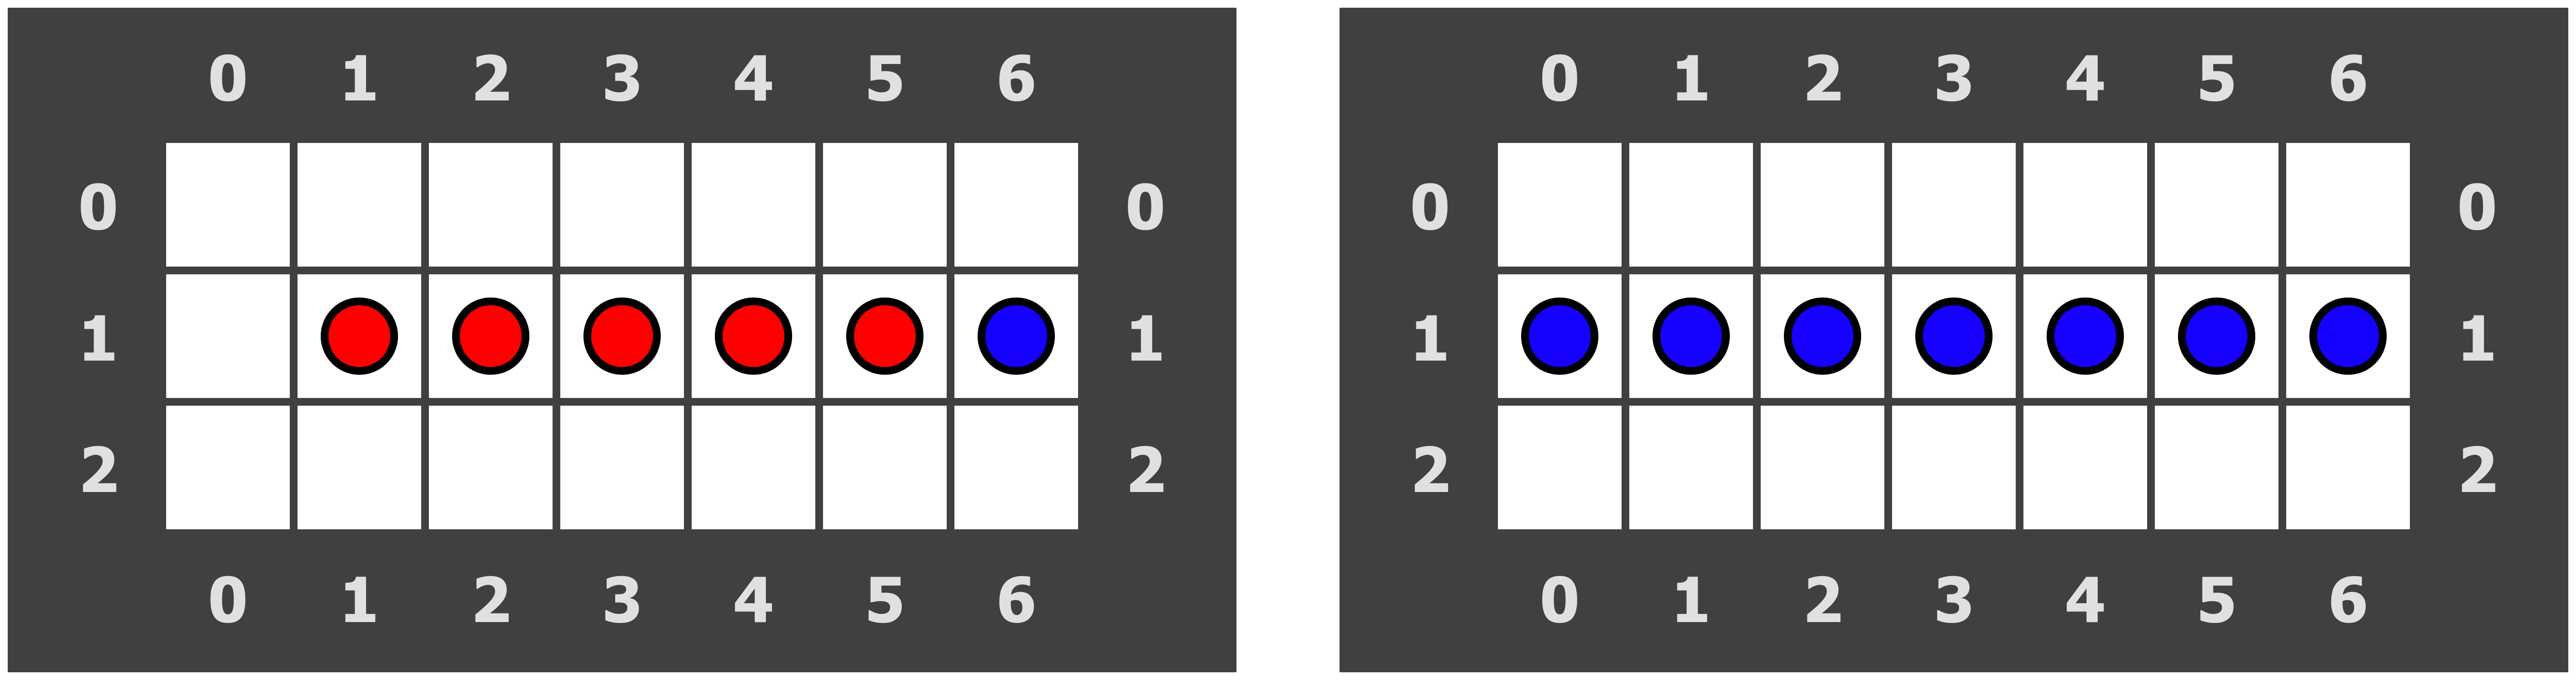
\includegraphics[width=0.6\linewidth]{pics/naive-game-situation}
    \captionof{figure}[Spielfeldsituation 01]{Problematik der naiven Bewertung}
    \label{fig:naivespielfeld01}
\end{minipage}

\subsection{Bestandteile und Implementierung}\label{subsec:bestandteile-und-implementierung}
Wie bereits in der Einleitung gezeigt, gen\"ugt das reine Abz\"ahlen der Spielsteine nicht aus.
Deshalb setzen wir auf drei unterschiedliche Heuristiken, um die aktuelle Spielsituation zu bewerten.
Unter diesen drei Ans\"atzen werden die Mobilit\"at der Spieler, das Verh\"altnis der Spielsteine sowie die aktuelle Bewertung der Karte miteinbezogen.
Diese einzelnen Bestandteile sind w\"ahrend dem Spiel jedoch nicht immer gleichbedeutend, da zum Beispiel im fr\"uhen Spielverlauf die Mobilit\"at und das Besetzen von wichtigen Feldern von Vorteil ist.
Im sp\"ateren Spielverlauf m\"ussen die einzelnen Bestandteile anders gewertet werden.
Hierbei muss darauf geachtet werden, seine Anzahl an Steinen zu erh\"ohen.

\subsubsection{Gewichtung des Spielfeldes}
Es gibt gewisse Positionen die f\"ur einen Spieler wertvoller sind als andere.
Zu diesen Positionen z\"ahlen unter anderem Kanten und Ecken, da es wesentlich schwieriger, bis garnicht m\"oglich ist, diese einzunehmen.
Eine Ausnahme stellt hier das Einnehmen mithilfe von \"Uberschreib-, bzw.\ Spezialsteine dar.
Insbesondere sind Felder die zwei Felder oder mehr von einem Bonusfeld in direkter Richtung entfernt sind h\"oher gewichtet, da sie die M\"oglichkeit geben einen solchen Bonusstein einzunehmen falls ein Gegner auf ein direktes Nachbarfeld des Spezialfeldes zieht.

\vspace{1em}
\begin{minipage}{\linewidth}
    \centering
    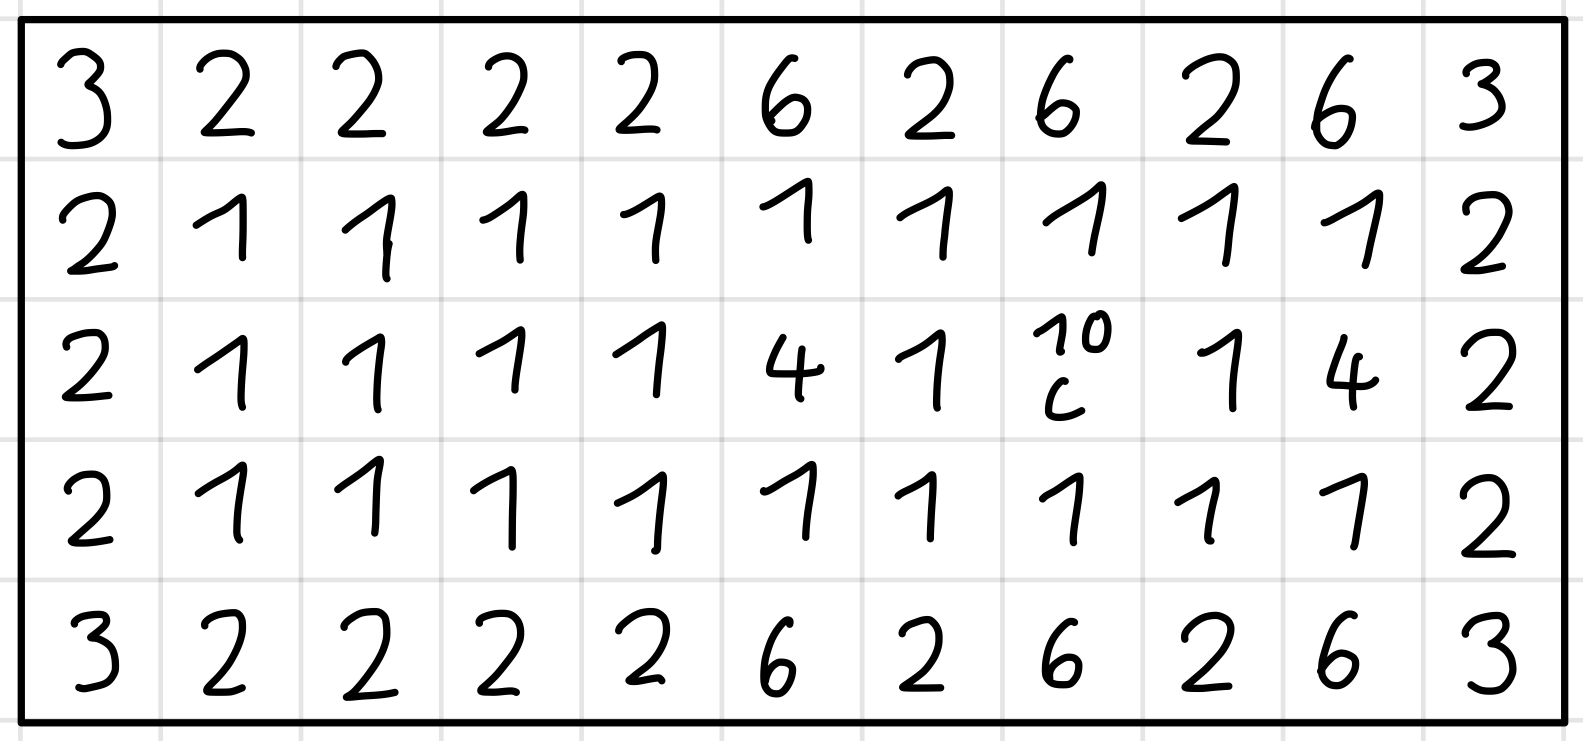
\includegraphics[width=0.5\linewidth]{pics/rating}
    \captionof{figure}[Bewertungsverfahren 01]{Spielfeldpositionen mit Gewichtungen}
    \label{fig:bewertungsverfahren01}
\end{minipage}

Der Score eines Spielers setzt sich dann aus der Summe der belegten Felder mit der entsprechenden Gewichtung zusammen.

Dieses Bewertungsverfahren bietet Vor- und Nachteile.
Positiv daran ist, dass bei Beginn des Spieles jedem Feld eine Gewichtung zugeteilt wird und diese nur noch durch erreichen von Spezialfeldern geringf\"ugig ge\"andert wird.
Negativ ist jedoch, dass dieses Bewertungsverfahren besonders bei gro"sen rechteckigen Spielfeldern mit wenig Spezialfeldern ann\"ahernd wie die naive Variante funktioniert.

\subsubsection{Mobilit\"at}
Ein weiterer Bestandteil der Analyse besteht darin, Spielsituationen anhand der Beweglichkeit der Spieler einzustufen.
Hierbei wird die Anzahl an Spielz\"ugen eines jeden Spielers bestimmt und miteinander verglichen.
Wie bereits in der Einleitung gezeigt kann ein Spieler seine positive Stellung nur halten, solange er weiterhin spielf\"ahig bleibt.
Aus diesem Grund wird in diesem Ansatz bestimmt wie beweglich ein Spieler gegen\"uber den Anderen ist.

Ein Vorteil dieser Bewertungsmethode besteht darin, dass ein Spieler mit wenig Steinen aber einer hohen Mobilit\"at bei diesem Verfahren nicht negativ bewertet wird.
Ein Problem daran ist jedoch, dass zum Ende des Spieles dieser Ansatz an Relevanz verliert, da zum Schluss nur die Anzahl an eigenen Steinen wichtig ist.

\subsubsection{Spielfeldbelegung}
Da es besonders gegen Ende des Spiels wichtig ist, viele Steine zu besitzen, muss man dies ebenfalls in die Bewertung miteinbeziehen.
Anstatt aber nur einfach die Anzahl der Spielsteine zu z\"ahlen, wird hier das prozentuale Verh\"altnis gegen\"uber allen existierenden Spielsteinen genommen.

Der Vorteil dieses Verfahrens ist hier, dass man vor allem im sp\"ateren Spielverlauf feststellen kann, wie der aktuelle Stand des Spiels ist und welche Spieler es anzugreifen gilt.
Der Nachteil hierbei ist aber, dass dieses Verfahren im anf\"anglichen und mittleren Spielverlauf nicht aussagekr\"aftig ist.
Allerdings muss man diese Berechnung wie Anfangs erw\"ahnt mit einflie"sen lassen, da man zum Schluss einen Greedyansatz w\"ahlen muss.
Denn letztlich ist f\"ur das Gewinnen des Spieles nur die Anzahl an Spielsteinen von Bedeutung.


\bigskip
\newpage